% Created by tikzDevice version 0.12.6 on 2026-05-14 21:28:34
% !TEX encoding = UTF-8 Unicode
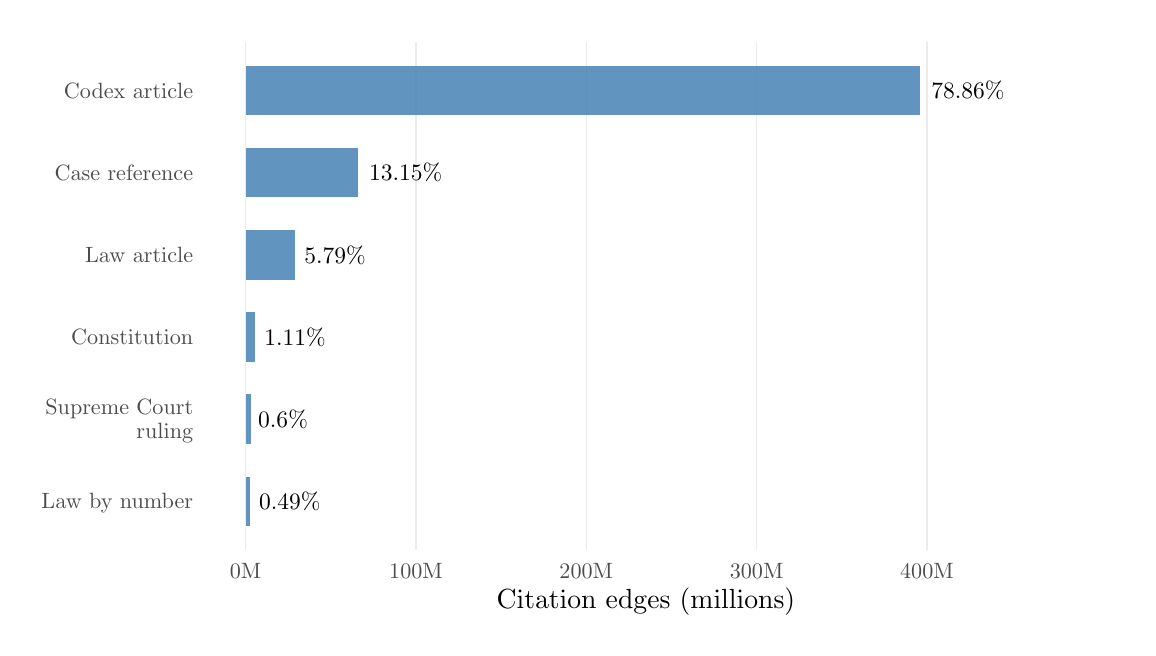
\begin{tikzpicture}[x=1pt,y=1pt]
\definecolor{fillColor}{RGB}{255,255,255}
\path[use as bounding box,fill=fillColor,fill opacity=0.00] (0,0) rectangle (397.48,216.81);
\begin{scope}
\path[clip] (  0.00,  0.00) rectangle (397.48,216.81);
\definecolor{fillColor}{RGB}{255,255,255}

\path[fill=fillColor] (  0.00,  0.00) rectangle (397.48,216.81);
\end{scope}
\begin{scope}
\path[clip] ( 64.29, 27.90) rectangle (382.48,211.81);
\definecolor{drawColor}{gray}{0.92}

\path[draw=drawColor,line width= 0.5pt,line join=round] ( 78.75, 27.90) --
	( 78.75,211.81);

\path[draw=drawColor,line width= 0.5pt,line join=round] (140.30, 27.90) --
	(140.30,211.81);

\path[draw=drawColor,line width= 0.5pt,line join=round] (201.84, 27.90) --
	(201.84,211.81);

\path[draw=drawColor,line width= 0.5pt,line join=round] (263.39, 27.90) --
	(263.39,211.81);

\path[draw=drawColor,line width= 0.5pt,line join=round] (324.94, 27.90) --
	(324.94,211.81);
\definecolor{fillColor}{RGB}{70,130,180}

\path[fill=fillColor,fill opacity=0.85] ( 78.75,185.11) rectangle (322.53,202.91);

\path[fill=fillColor,fill opacity=0.85] ( 78.75,155.45) rectangle (119.39,173.25);

\path[fill=fillColor,fill opacity=0.85] ( 78.75,125.79) rectangle ( 96.64,143.58);

\path[fill=fillColor,fill opacity=0.85] ( 78.75, 96.12) rectangle ( 82.18,113.92);

\path[fill=fillColor,fill opacity=0.85] ( 78.75, 66.46) rectangle ( 80.60, 84.26);

\path[fill=fillColor,fill opacity=0.85] ( 78.75, 36.80) rectangle ( 80.27, 54.59);
\definecolor{drawColor}{RGB}{0,0,0}

\node[text=drawColor,anchor=base west,inner sep=0pt, outer sep=0pt, scale=  0.85] at (326.51,191.07) {78.86\%};

\node[text=drawColor,anchor=base west,inner sep=0pt, outer sep=0pt, scale=  0.85] at (123.37,161.41) {13.15\%};

\node[text=drawColor,anchor=base west,inner sep=0pt, outer sep=0pt, scale=  0.85] at ( 99.98,131.75) {5.79\%};

\node[text=drawColor,anchor=base west,inner sep=0pt, outer sep=0pt, scale=  0.85] at ( 85.52,102.08) {1.11\%};

\node[text=drawColor,anchor=base west,inner sep=0pt, outer sep=0pt, scale=  0.85] at ( 83.30, 72.42) {0.6\%};

\node[text=drawColor,anchor=base west,inner sep=0pt, outer sep=0pt, scale=  0.85] at ( 83.61, 42.75) {0.49\%};
\end{scope}
\begin{scope}
\path[clip] (  0.00,  0.00) rectangle (397.48,216.81);
\definecolor{drawColor}{gray}{0.30}

\node[text=drawColor,anchor=base east,inner sep=0pt, outer sep=0pt, scale=  0.80] at ( 59.79, 42.94) {Law by number};

\node[text=drawColor,anchor=base east,inner sep=0pt, outer sep=0pt, scale=  0.80] at ( 59.79, 76.92) {Supreme Court};

\node[text=drawColor,anchor=base east,inner sep=0pt, outer sep=0pt, scale=  0.80] at ( 59.79, 68.28) {ruling};

\node[text=drawColor,anchor=base east,inner sep=0pt, outer sep=0pt, scale=  0.80] at ( 59.79,102.27) {Constitution};

\node[text=drawColor,anchor=base east,inner sep=0pt, outer sep=0pt, scale=  0.80] at ( 59.79,131.93) {Law article};

\node[text=drawColor,anchor=base east,inner sep=0pt, outer sep=0pt, scale=  0.80] at ( 59.79,161.59) {Case reference};

\node[text=drawColor,anchor=base east,inner sep=0pt, outer sep=0pt, scale=  0.80] at ( 59.79,191.26) {Codex article};
\end{scope}
\begin{scope}
\path[clip] (  0.00,  0.00) rectangle (397.48,216.81);
\definecolor{drawColor}{gray}{0.30}

\node[text=drawColor,anchor=base,inner sep=0pt, outer sep=0pt, scale=  0.80] at ( 78.75, 17.89) {0M};

\node[text=drawColor,anchor=base,inner sep=0pt, outer sep=0pt, scale=  0.80] at (140.30, 17.89) {100M};

\node[text=drawColor,anchor=base,inner sep=0pt, outer sep=0pt, scale=  0.80] at (201.84, 17.89) {200M};

\node[text=drawColor,anchor=base,inner sep=0pt, outer sep=0pt, scale=  0.80] at (263.39, 17.89) {300M};

\node[text=drawColor,anchor=base,inner sep=0pt, outer sep=0pt, scale=  0.80] at (324.94, 17.89) {400M};
\end{scope}
\begin{scope}
\path[clip] (  0.00,  0.00) rectangle (397.48,216.81);
\definecolor{drawColor}{RGB}{0,0,0}

\node[text=drawColor,anchor=base,inner sep=0pt, outer sep=0pt, scale=  1.00] at (223.39,  6.94) {Citation edges (millions)};
\end{scope}
\end{tikzpicture}
